
\documentclass[12pt]{article}
\usepackage{graphicx}
\usepackage{hyperref}
\usepackage[activate={true,nocompatibility},final,tracking=true,kerning=true,spacing=nonfrench,factor=1100,stretch=15,shrink=15]{microtype}
\SetTracking{encoding={*}, shape=sc}{0}

%%%%%%%%%%%%%%%%%%%%%%%%%%%%%%%%%%%%%%%%%%%%%%%%%%%%%%%%%%%%%%%%%%%%
% basic data for the eprint:
%%%%%%%%%%%%%%%%%%%%%%%%%%%%%%%%%%%%%%%%%%%%%%%%%%%%%%%%%%%%%%%%%%%%

\textwidth=6.0in  \textheight=8.25in

%%  Adjust these for your printer:
\leftmargin=-0.3in   \topmargin=-0.20in

%% preprint number data:
\newcommand\pubnumber{}
\newcommand\pubdate{\today}

%%  address and funding acknowledgement data:
\def\institute{Centre for Cosmology, Particle Physics and Phenomenology\\
Universit\'e catholique de Louvain, B-1348 Louvain-la-Neuve, BELGIUM}
\def\support{\footnote{Work supported by Fonds de la Recherche Scientifique (FNRS), Belgium.}}

%%%%%%%%%%%%%%%%%%%%%%%%%%%%%%%%%%%%%%%%%%%%%%%%%%%%%%%%%%%%%%%%%%%%%%%%%%%%
%   document style macros
%%%%%%%%%%%%%%%%%%%%%%%%%%%%%%%%%%%%%%%%%%%%%%%%%%%%%%%%%%%%%%%%%%%%%%%%%%%%
\def\Title#1{\begin{center} {\Large #1 } \end{center}}
\def\Author#1{\begin{center}{ \sc #1} \end{center}}
\def\Address#1{\begin{center}{ \it #1} \end{center}}
\def\andauth{\begin{center}{and} \end{center}}
\def\submit#1{\begin{center}Submitted to {\sl #1} \end{center}}
\newcommand\pubblock{\rightline{\begin{tabular}{l} \pubnumber\\
         \pubdate  \end{tabular}}}
\newenvironment{Abstract}{\begin{quotation}  }{\end{quotation}}
\newenvironment{Presented}{\begin{quotation} \begin{center} 
             PRESENTED AT\end{center}\bigskip 
      \begin{center}\begin{large}}{\end{large}\end{center} \end{quotation}}
\def\Acknowledgements{\bigskip  \bigskip \begin{center} \begin{large}
             \bf ACKNOWLEDGEMENTS \end{large}\end{center}}
%%%%%%%%%%%%%%%%%%%%%%%%%%%%%%%%%%%%%%%%%%%%%%%%%%%%%%%%%%%%%%%%%%%%%%%%%%%%
%  personal abbreviations and macros
%    the following package contains macros used in this document:
\input econfmacros.tex
%%%%%%%%%%%%%%%%%%%%%%%%%%%%%%%%%%%%%%%%%%%%%%%%%%%%%%%%%%%%%%%%%%%%%%%%%%%

\begin{document}
\begin{titlepage}
\pubblock

\vfill
\Title{Measurements of single top quark cross sections at 13~TeV with the CMS experiement}
\vfill
\Author{Matthias Komm\support}
\Address{\institute}
\vfill
\begin{Abstract}
An overview of recent measurements of inclusive and differential single top quark cross sections at 13~TeV with the CMS experiment is given in this note. This includes measurements targeting the $t$-channel and tW production modes resulting in inclusive cross sections of $\sigma_{t\mathrm{\mbox{-}ch.}}=$ and $\sigma_\mathrm{tW}=$ respectively. In addition, the $t$-channel cross section has been measured differentially as a function of the top quark transverse momentum and rapidity. Furthermore, a search for single top quark production in association with a Z~boson is detailed which yields an observed (expected) significance of 3.7 (3.1) standard deviations. 
\end{Abstract}
\vfill
\begin{Presented}
$10^{th}$ International Workshop on Top Quark Physics\\
Braga, Portugal,  September 17--22, 2017
\end{Presented}
\vfill
\end{titlepage}
\def\thefootnote{\fnsymbol{footnote}}
\setcounter{footnote}{0}
%

\section{Introduction}

The production mechanisms of single top quarks offer an experimental unique access to study details of electroweak interactions. For example, inclusive cross section measurements can be used to derive limits on the magnitude of the Cabibbo-Kobayashi-Maskawa (CKM) matrix element $\mathrm{V}_\mathrm{tb}$. Differential cross sections on the other hand allow to perform in-deep tests of the theoretical modeling and coupling structure. In this note recent measurements of single top quark production in $t$- and tW-channel as well as a search for tZq production by the CMS experiment at a center-of-mass energy of 13~TeV are presented.

\section{$t$-channel}

\begin{figure}[!htb]
\begin{center}
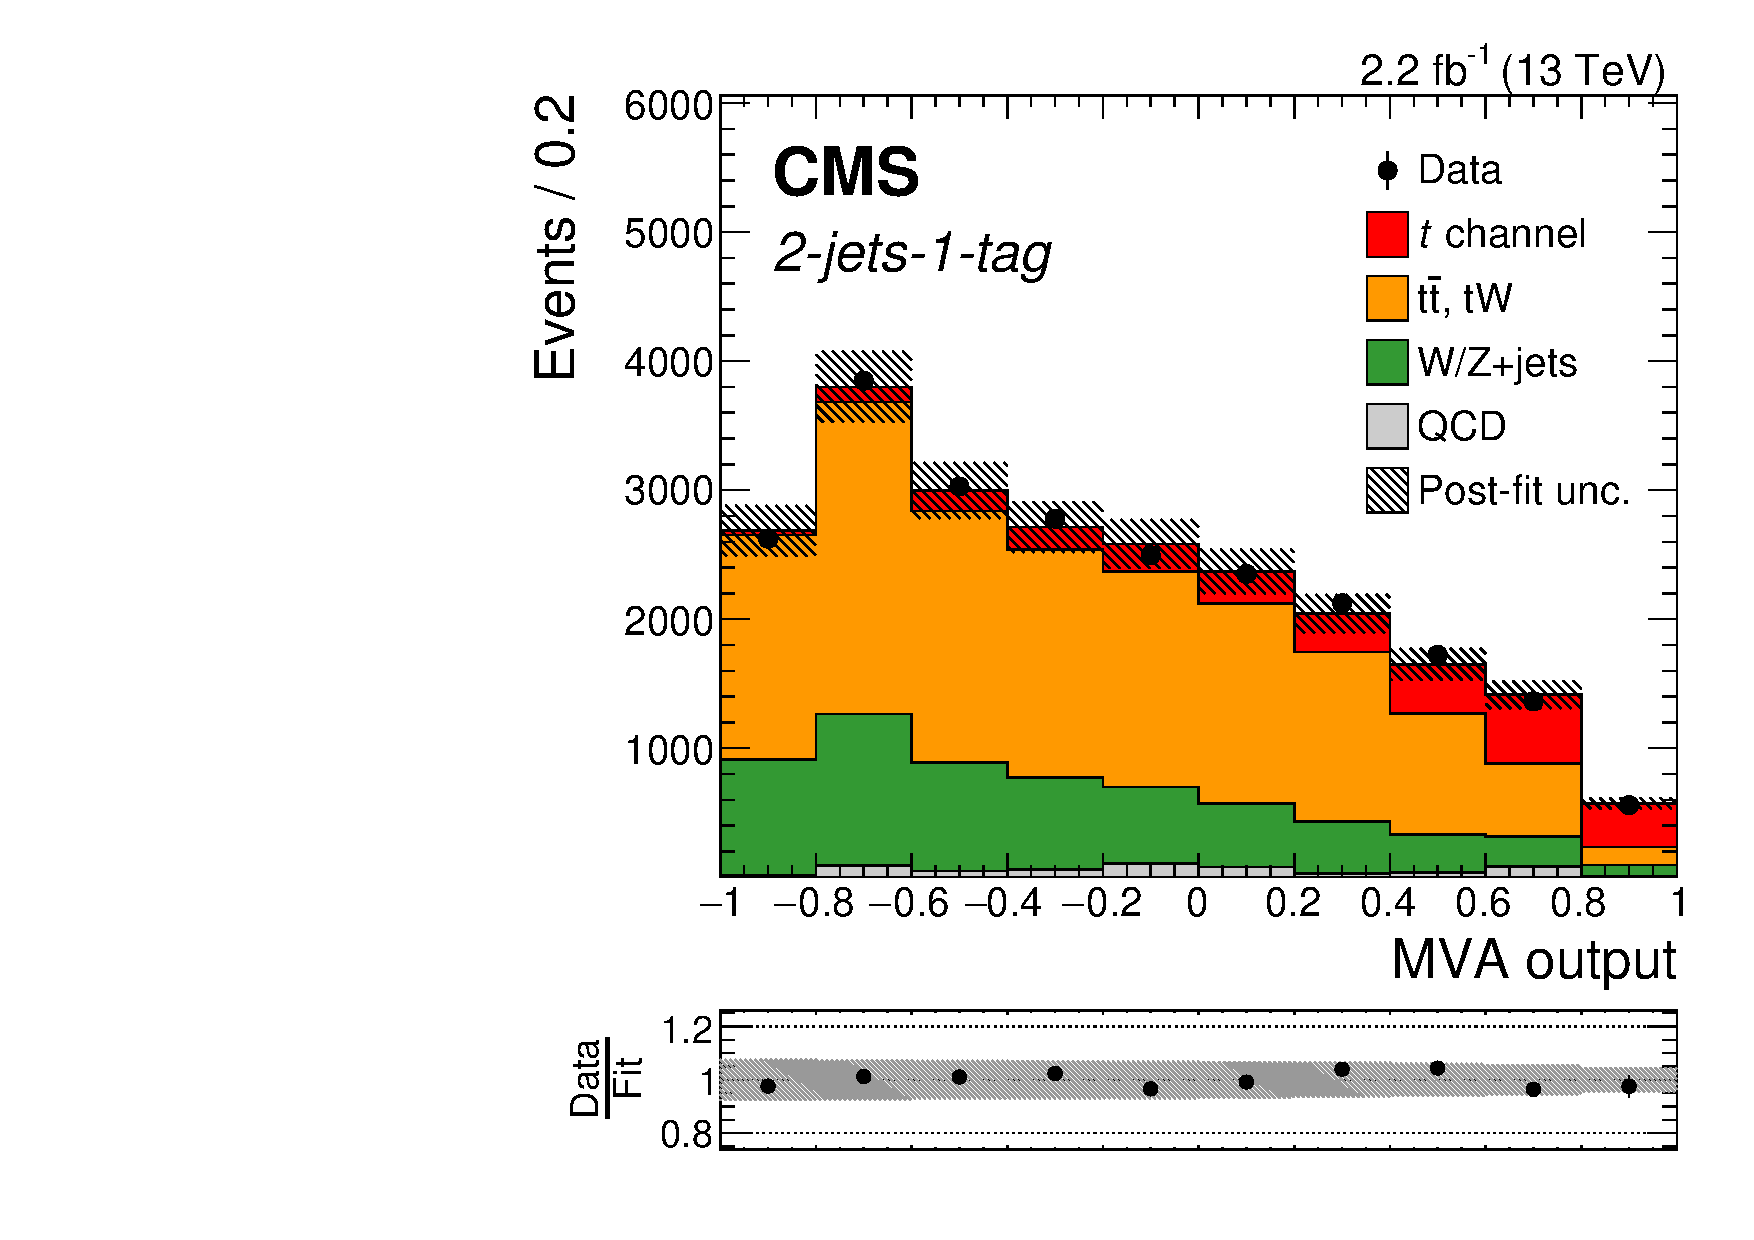
\includegraphics[width=0.38\textwidth]{tch-nn.pdf}\hspace{0.02\textwidth}
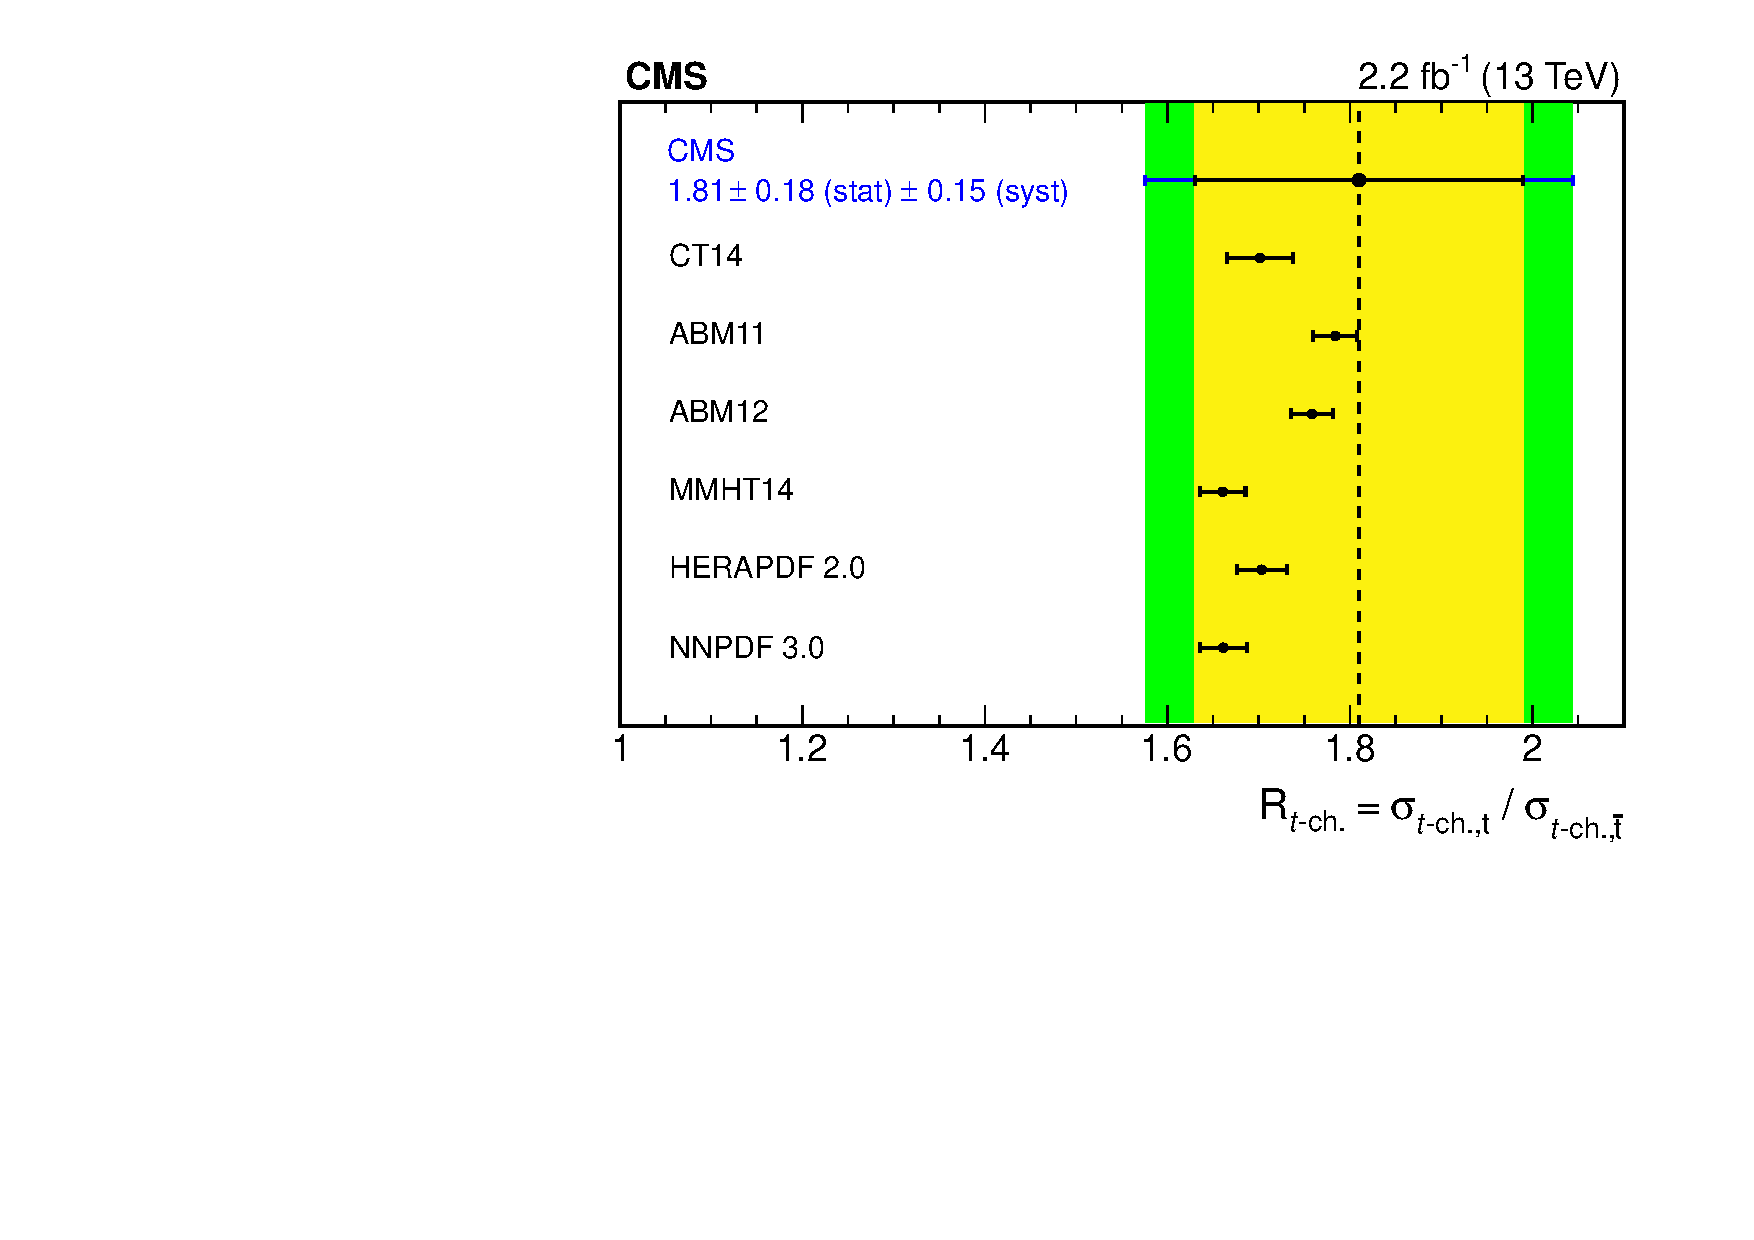
\includegraphics[width=0.55\textwidth]{tch-ratio.pdf}
\caption{Measurement of inclusive $t$-channel cross section: (left)~distribution of neural network discriminant for fitting; (right)~measured charge ratio compared to various PDF sets. The figures are taken from Ref~\cite{tchannel-inc}.}
\end{center}
\end{figure}


\begin{figure}[!htb]
\begin{center}
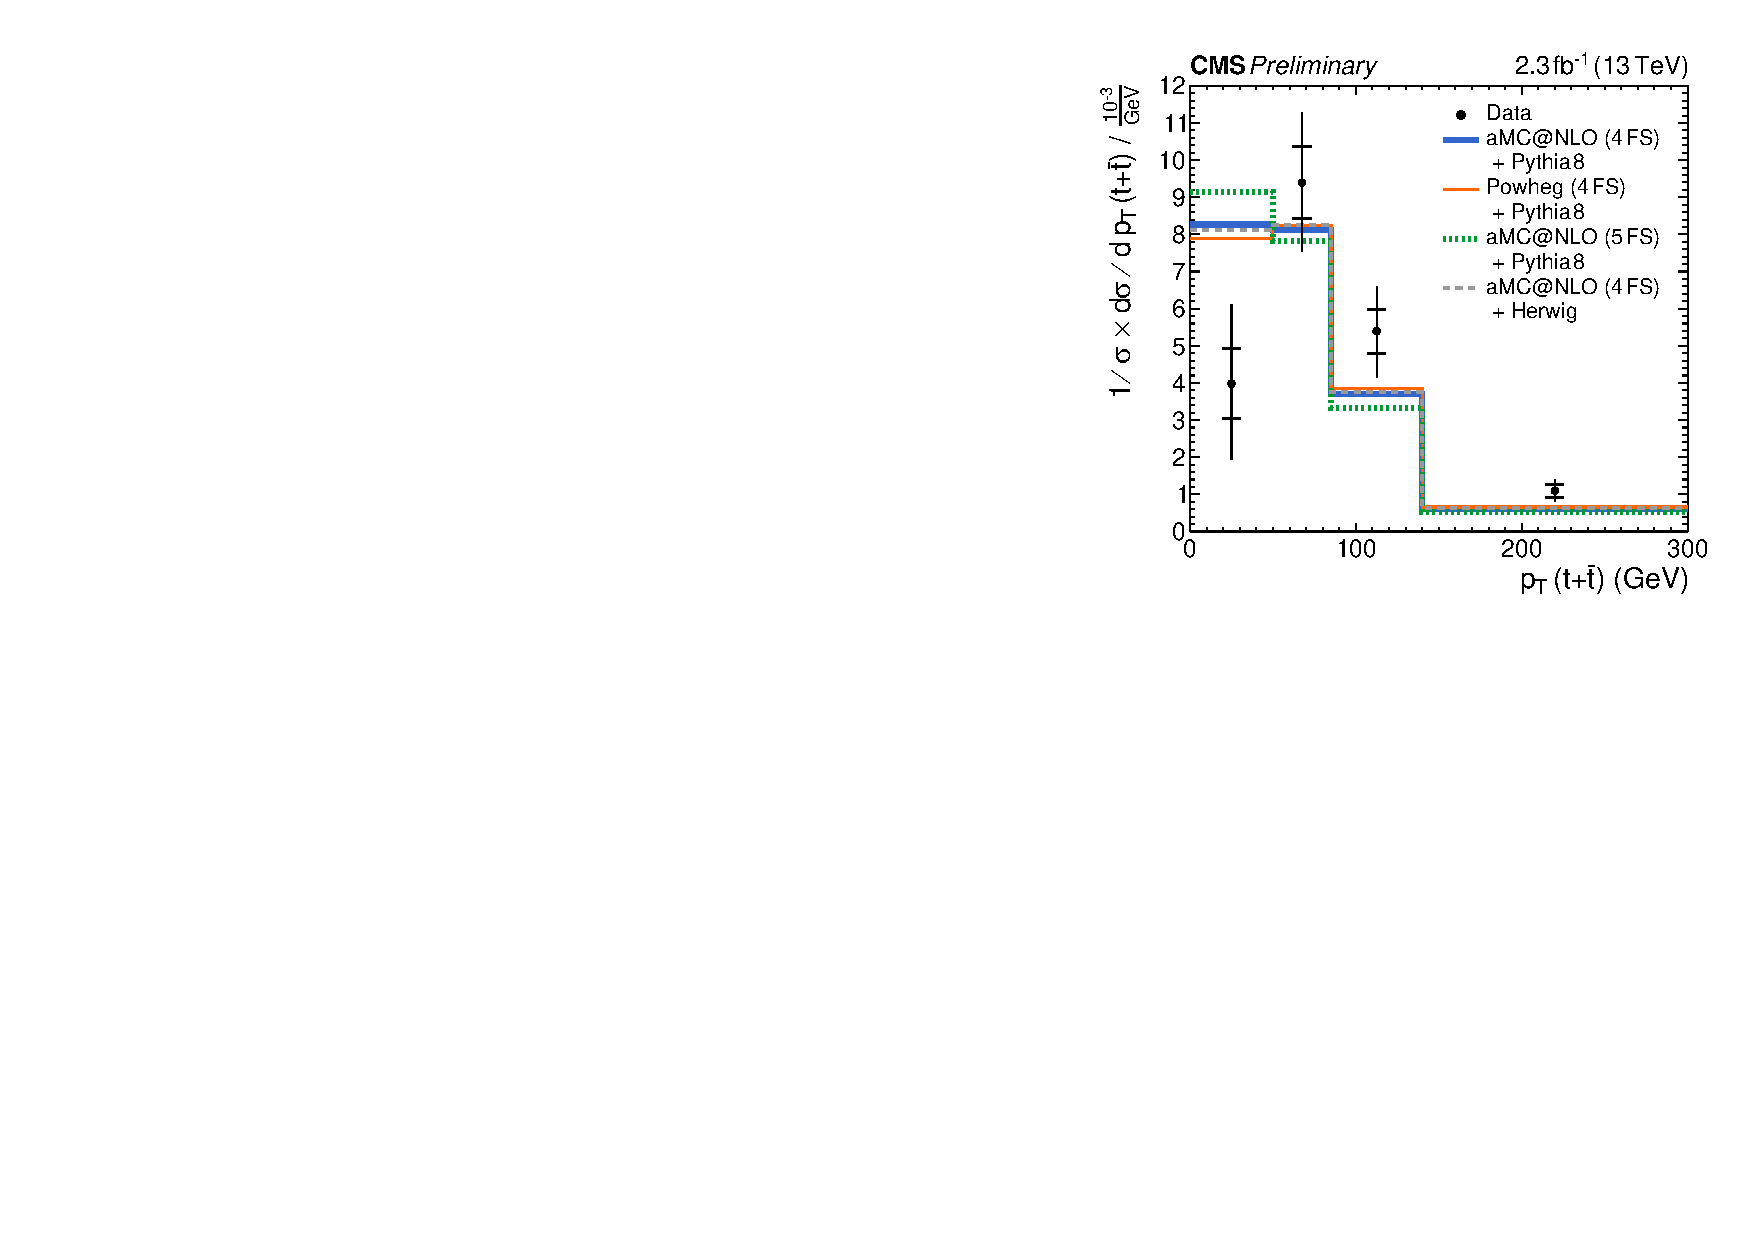
\includegraphics[width=0.45\textwidth]{unfolded_top_pt.pdf}\hspace{0.02\textwidth}
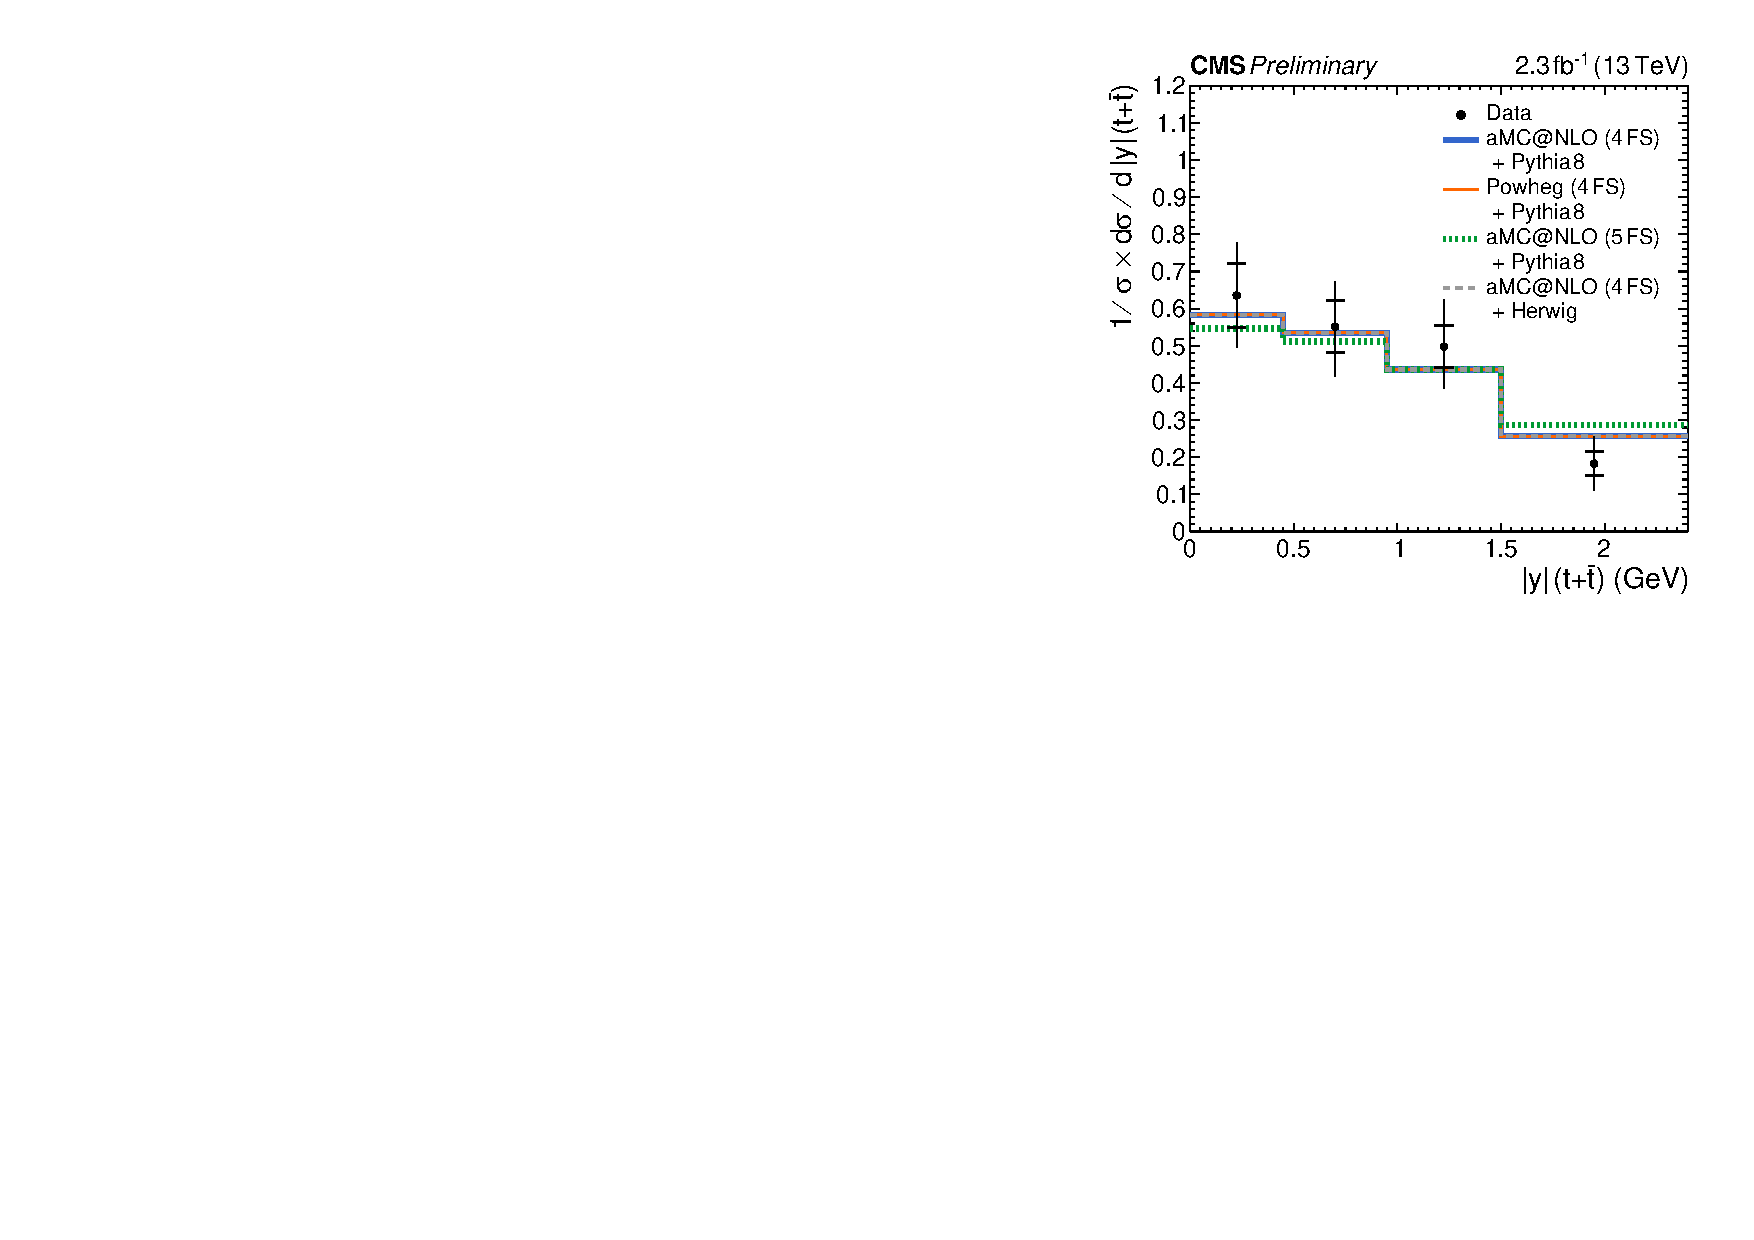
\includegraphics[width=0.45\textwidth]{unfolded_top_y.pdf}
\caption{Measurement of differential $t$-channel cross section as a function of the top quark (left)~transverse momentum and (right)~rapidity. The figures are taken from Ref~\cite{tchannel-diff}.}
\end{center}
\end{figure}

\section{tW-channel}

\begin{figure}[!htb]
\begin{center}
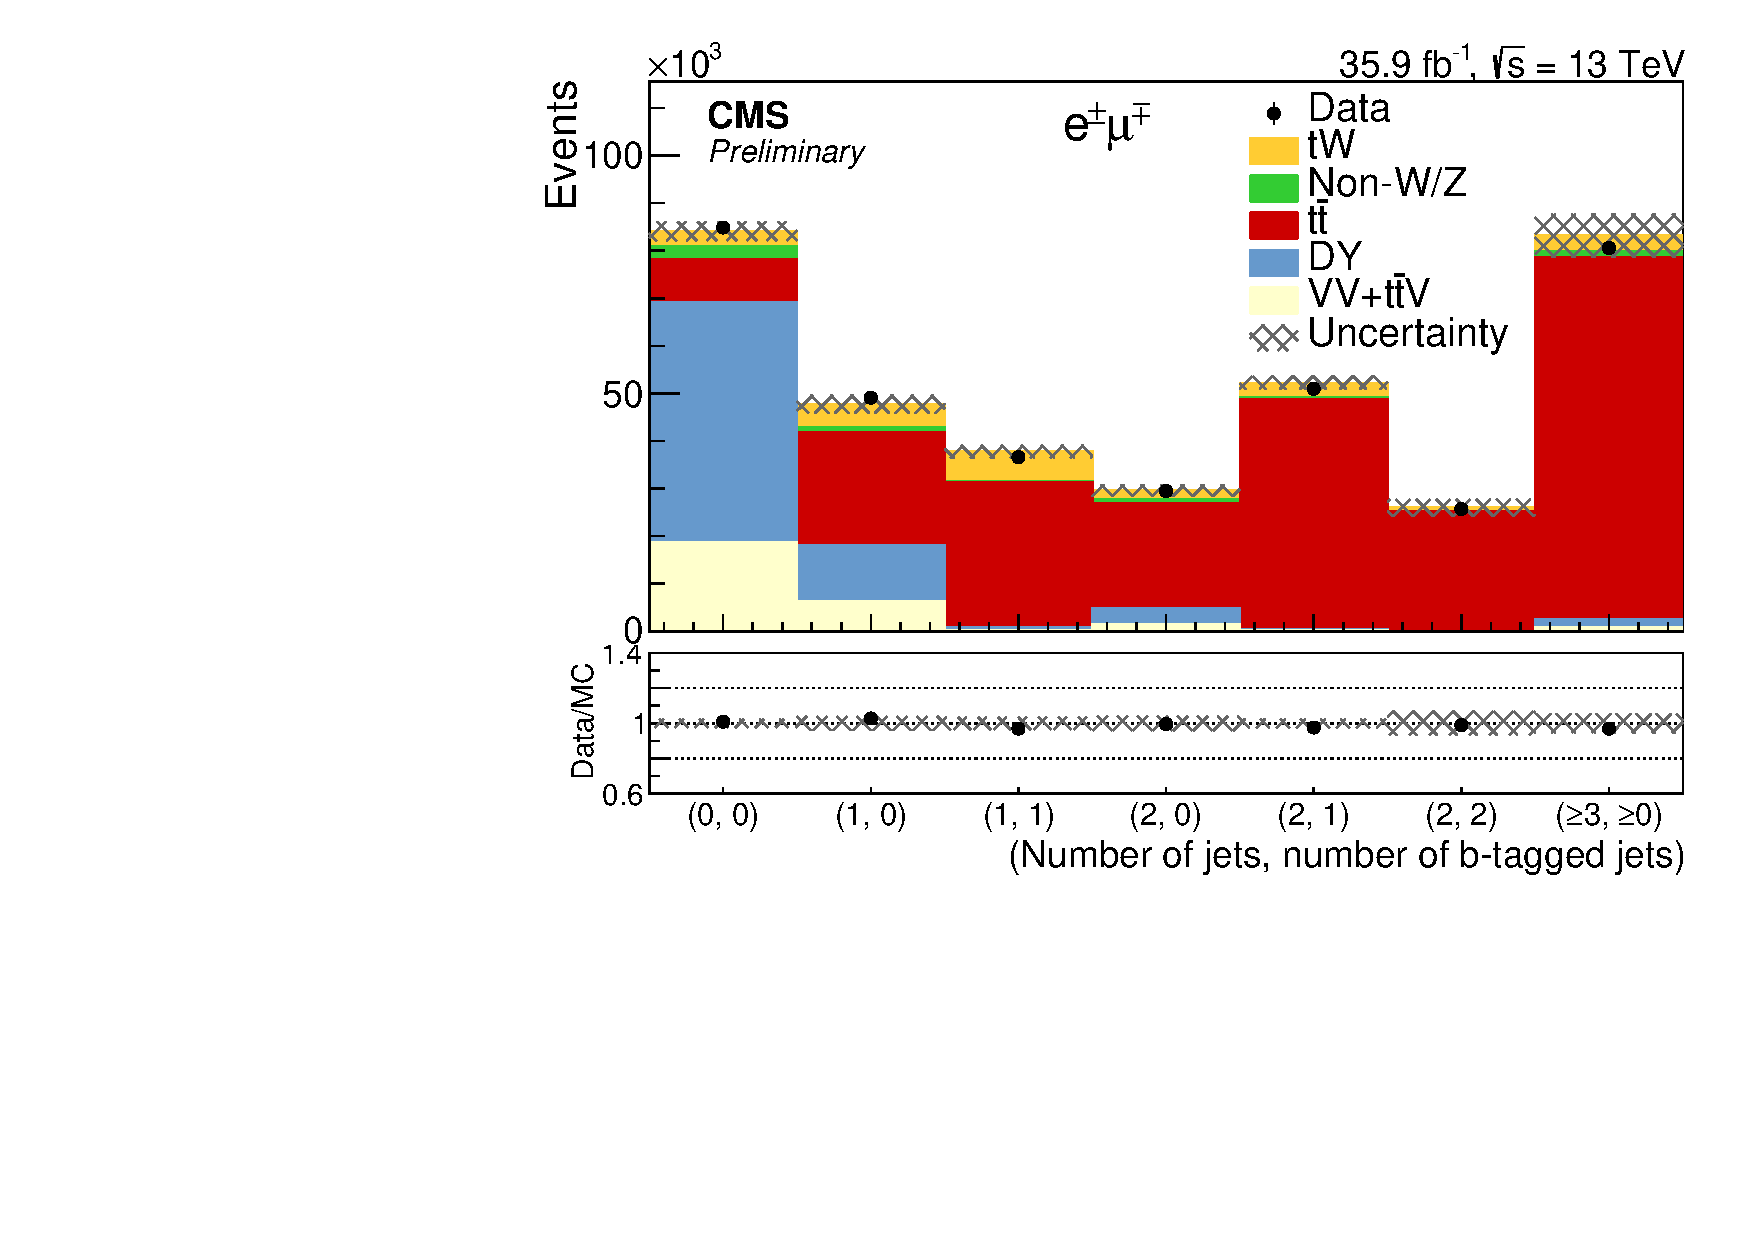
\includegraphics[width=0.47\textwidth]{tW-categories.pdf}\hspace{0.02\textwidth}
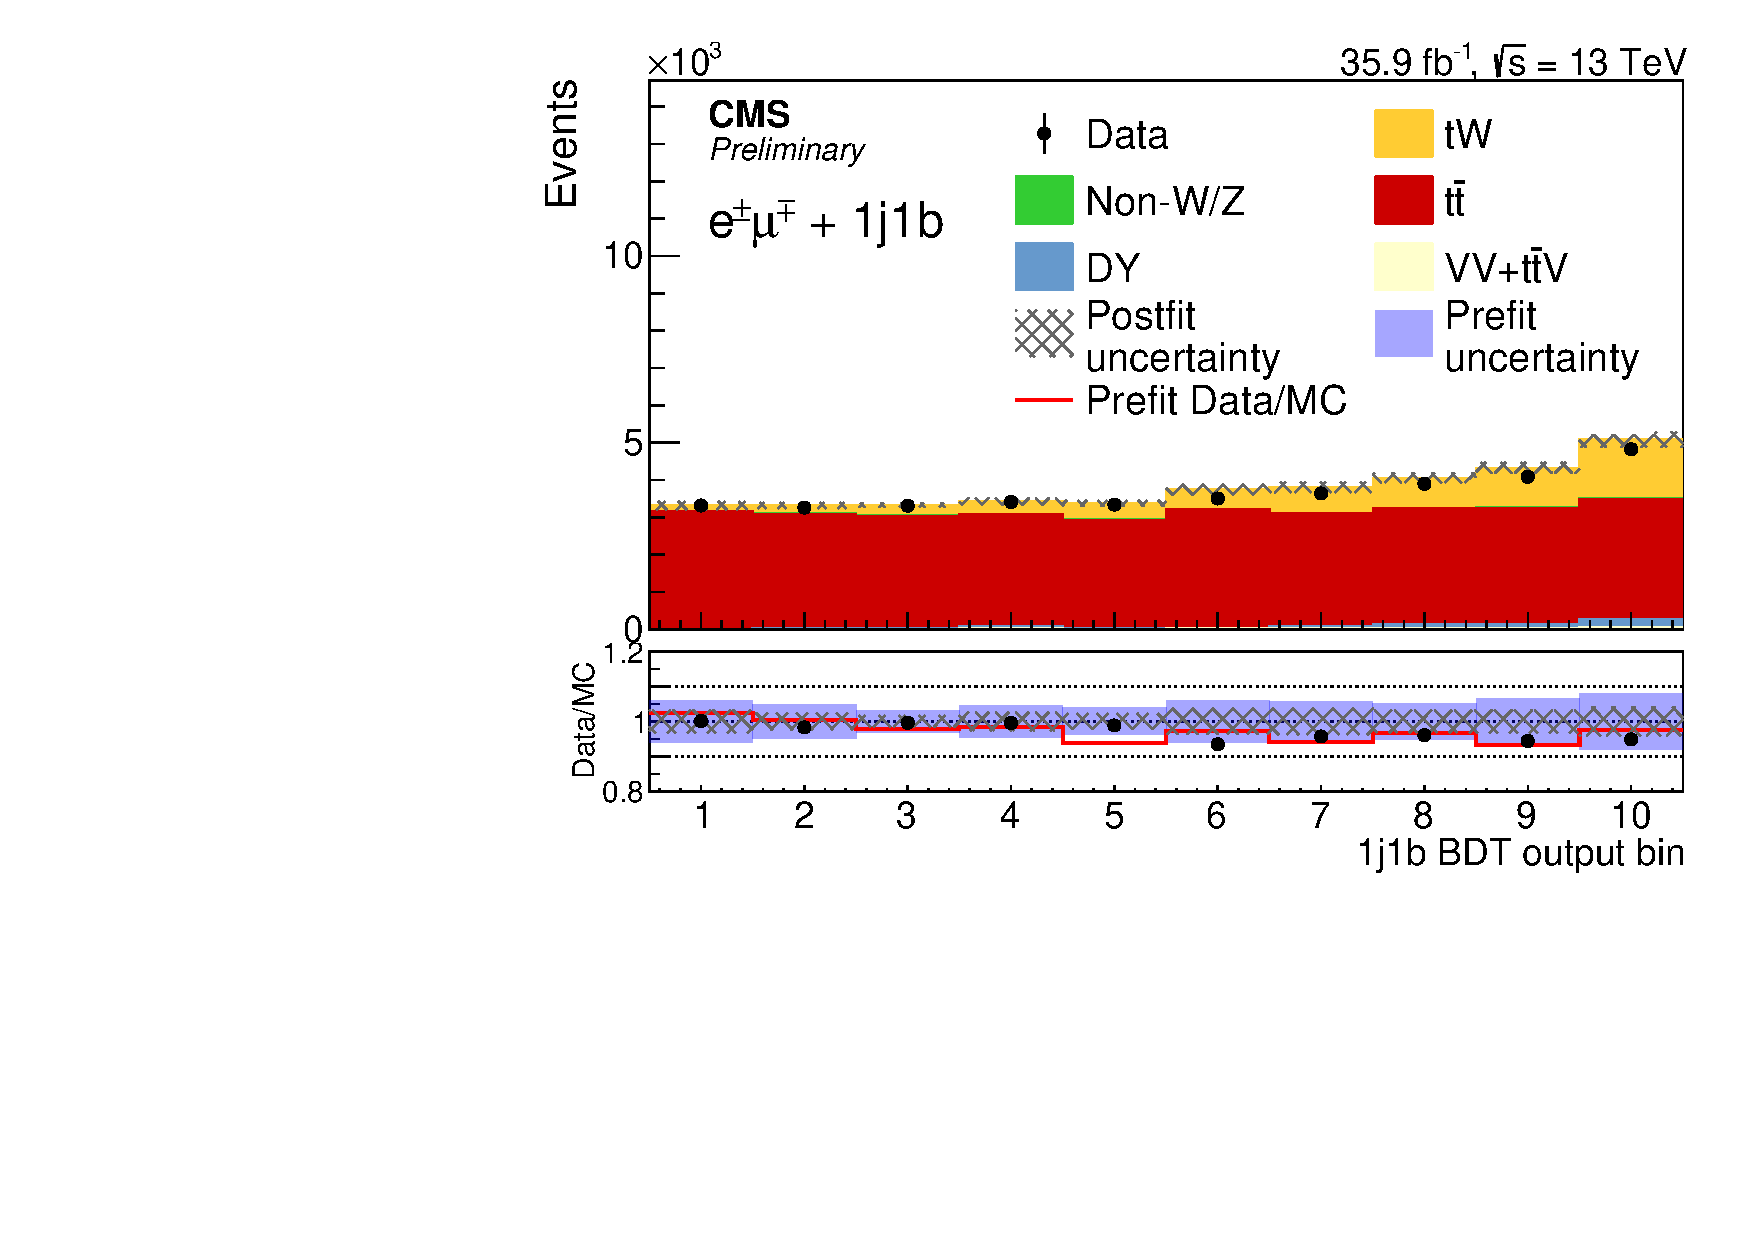
\includegraphics[width=0.47\textwidth]{tW-bdt.pdf}
\caption{Measurement of single top quark cross section in tW-channel: (left)~predicted and observed number of event per category; (right)~distribution of BDT discriminant in (1 jet, 1 b-tag)~category. The figures are taken from Ref~\cite{tw-inc}.}
\end{center}
\end{figure}

\section{tZq production}

\begin{figure}[!htb]
\begin{center}
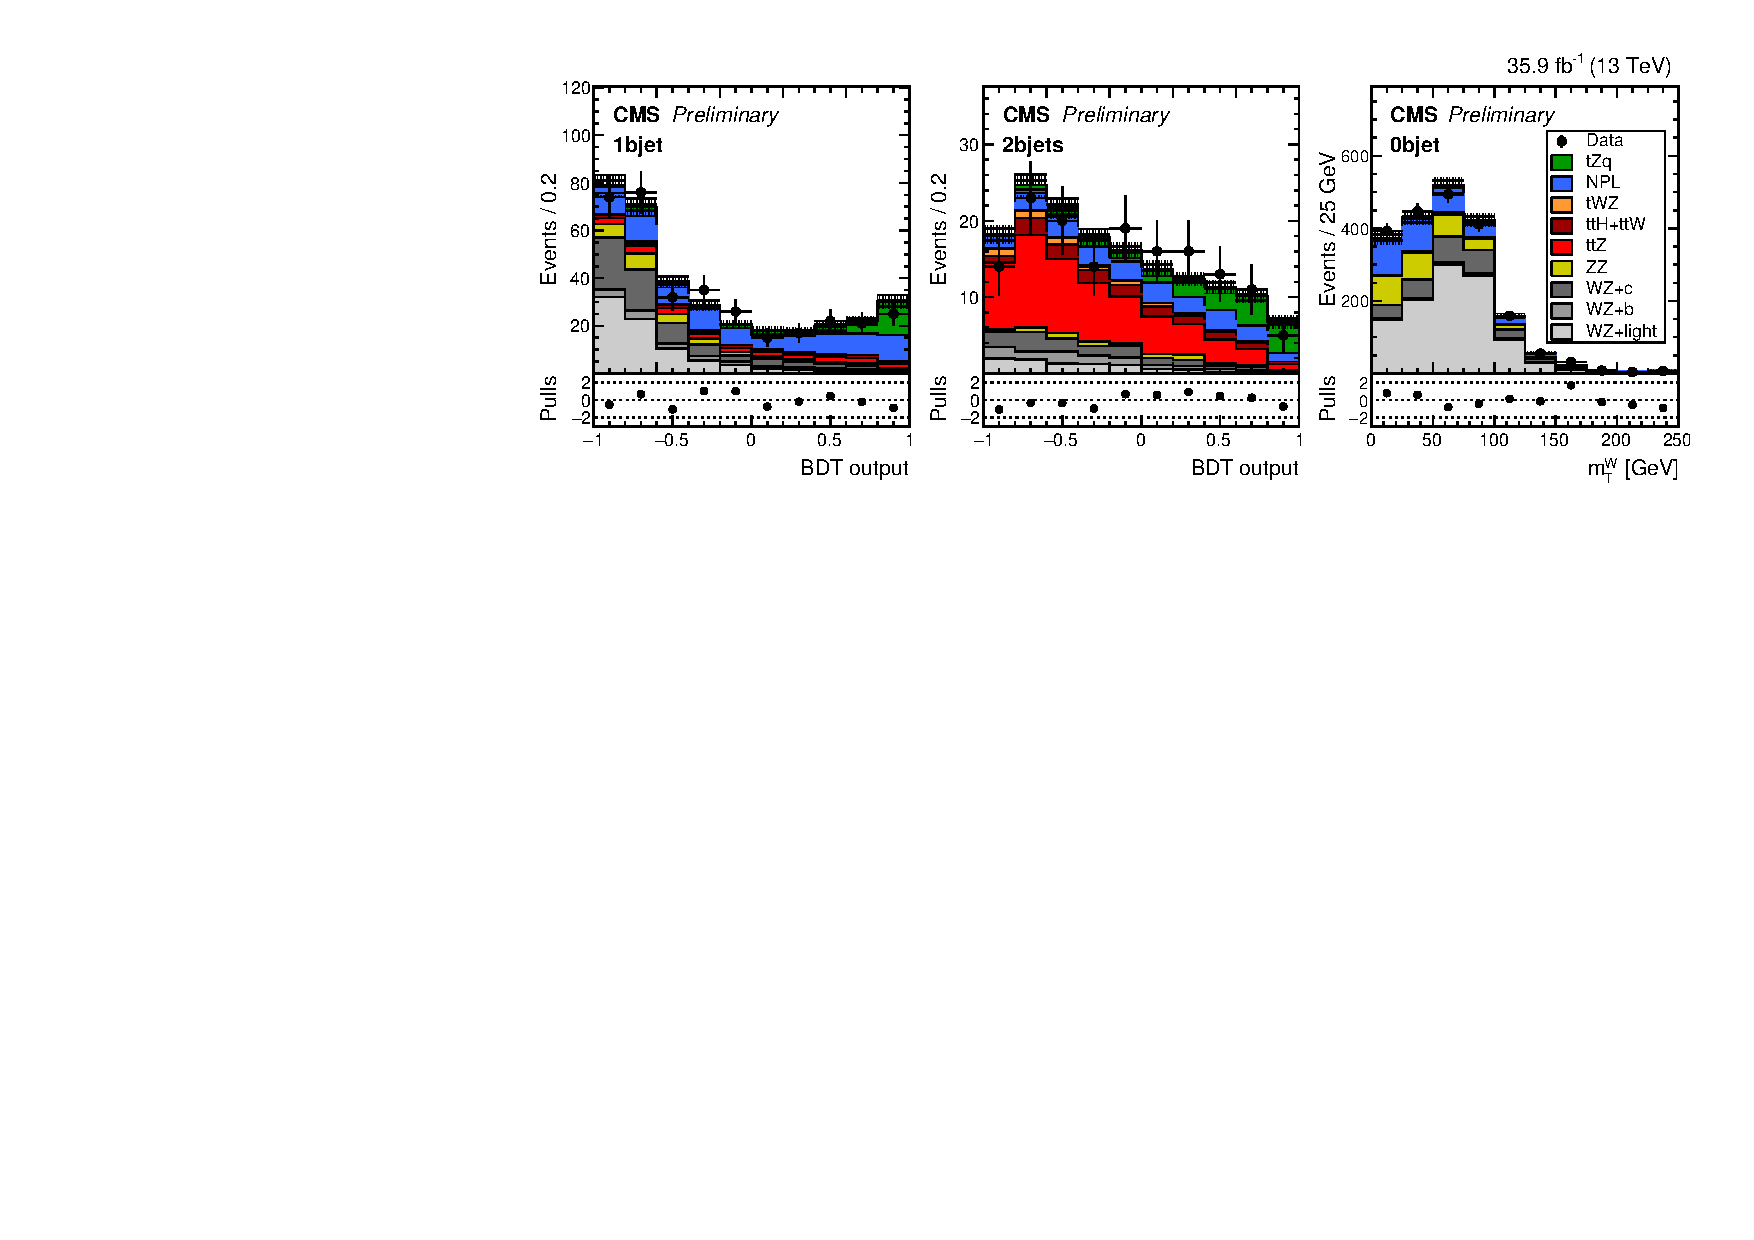
\includegraphics[width=0.97\textwidth]{tZq-fit.pdf}
\caption{Distributions of ??? . The figures are taken from Ref~\cite{tZq-inc}.}
\end{center}
\end{figure}

\section{Conclusion}

\begin{figure}[!htb]
\begin{center}
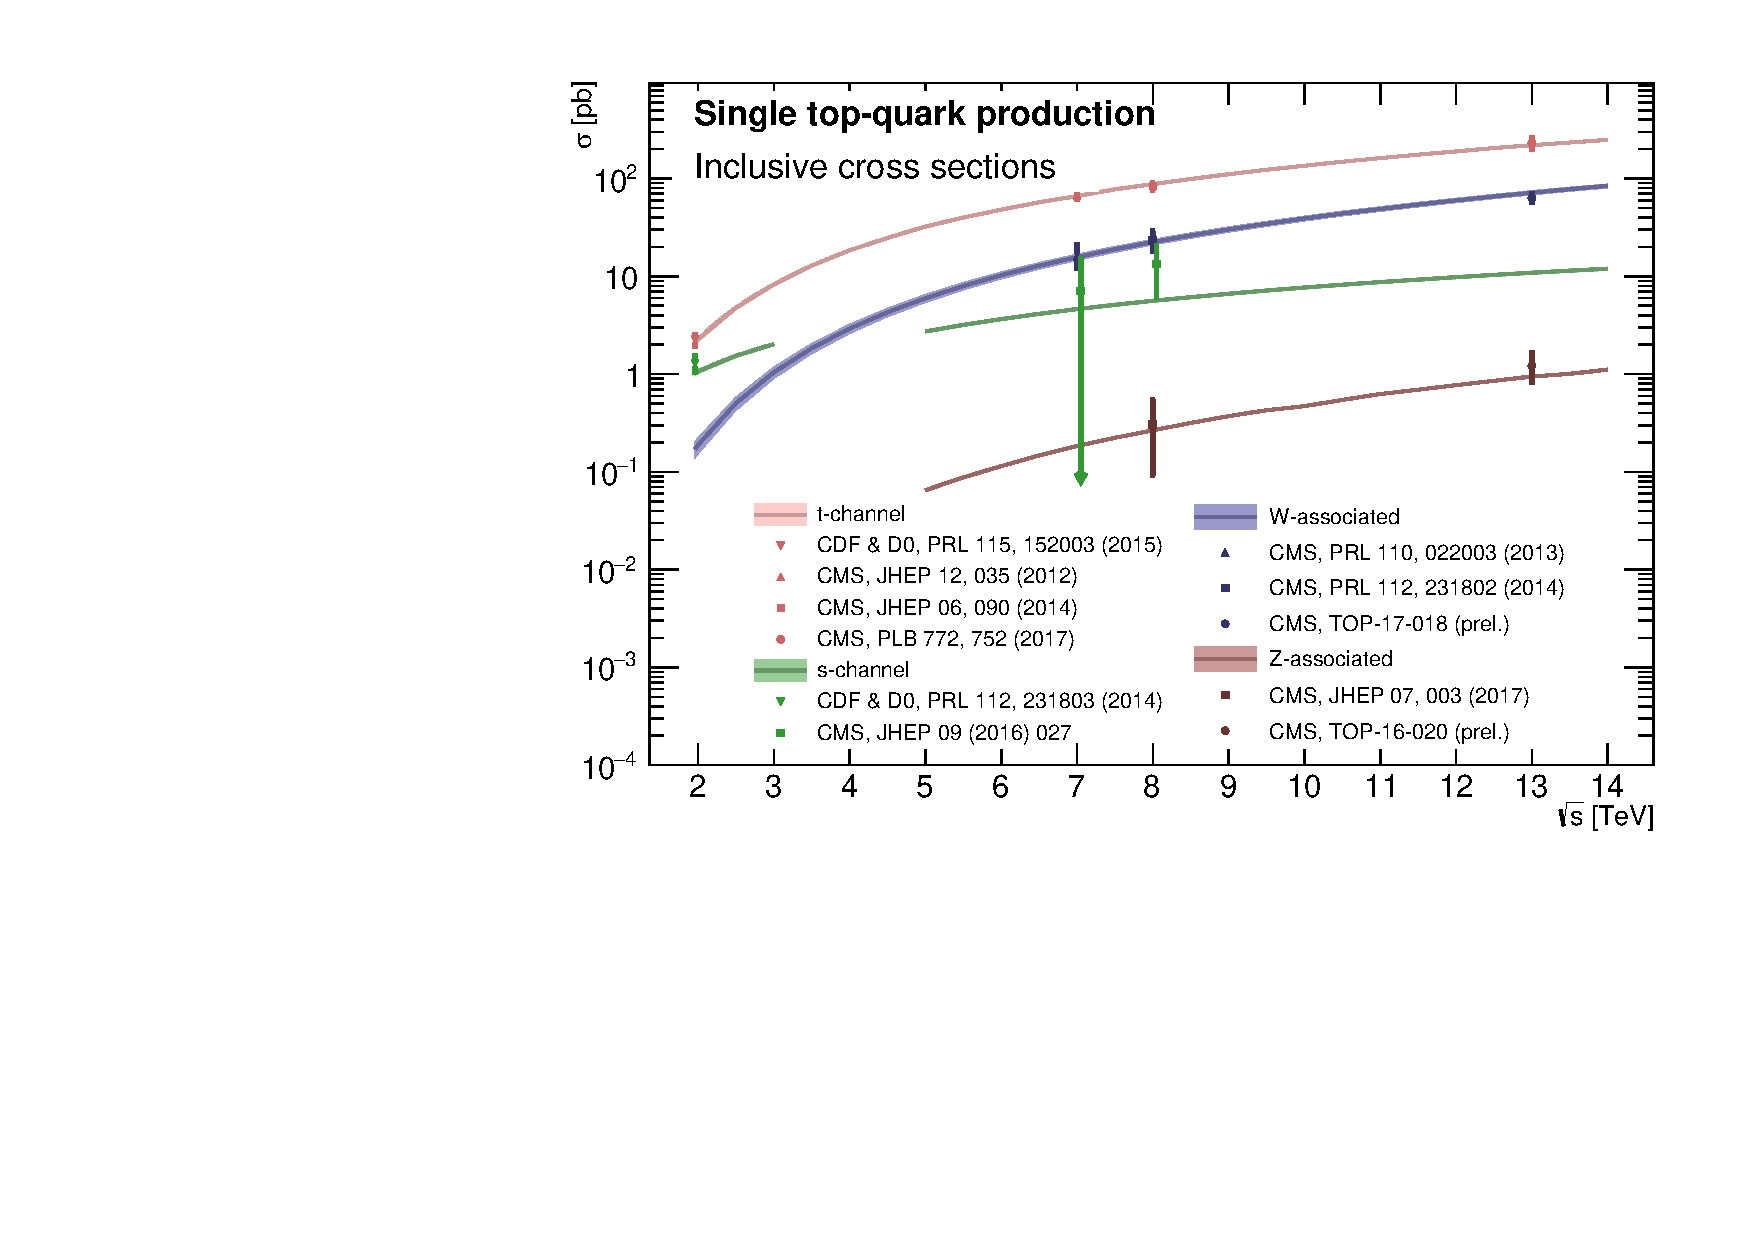
\includegraphics[width=0.7\textwidth]{singletopSep2017_noATLAS.pdf}
\caption{Overview of inclusive single top quark cross section measurements with the CMS experiment. The figure is adapted from Ref.~\cite{Giammanco}.}
\end{center}
\end{figure}

\begin{thebibliography}{99}

\bibitem{tchannel-inc}{CMS collaboration, Phys.Lett. \textbf{B772} (2017) 752--776.}
\bibitem{tchannel-diff}{CMS collaboration, CMS Physics Analysis Summary, CMS-PAS-TOP-16-004, 2016.}
\bibitem{tw-inc}{CMS collaboration, CMS Physics Analysis Summary, CMS-PAS-TOP-17-018, 2017.}
\bibitem{tZq-inc}{CMS collaboration, CMS Physics Analysis Summary, CMS-PAS-TOP-16-020, 2017.}
\bibitem{Giammanco}{A. Giammanco and R. Schwienhorst, \texttt{arXiv:1710.10699 [hep-ex]}.}


\end{thebibliography}

 
\end{document}

